\documentclass[11pt,a4paper]{article}

\usepackage[margin=1in]{geometry}
\usepackage{graphicx}
\usepackage{amsmath}
\usepackage{booktabs}
\usepackage{hyperref}
\usepackage[numbers]{natbib}

\title{Differentiable Cone-Beam CT Reconstruction\\
with Multi-Scale Voxel Embeddings}
\author{[Name]\\ COSC440}
\date{}

\begin{document}
\maketitle

\begin{abstract}
\noindent
[Placeholder: one paragraph. Differentiable rendering of a chest CBCT volume from 50 cone-beam projections. Model~1 uses nearest multi-scale embedding lookup. Model~2 replaces that lookup with trilinear interpolation of the same tables. State whether volumetric SSIM improved, stayed the same, or worsened by epoch~50. Absolute metric values are not the claim.]
\end{abstract}

\section{Introduction}
Differentiable rendering optimises a 3D scene so that rendered views match observed images~\cite{atlasprojectslides2026}.
This project reconstructs a monochromatic cone-beam CT (CBCT) volume from sparse projections using a simplified neural attenuation field~\cite{cosc440brief2026,zha2022naf}.
Geometry and projections come from the TIGRE toolbox~\cite{tigre}.

The baseline (Model~1) encodes query points on a power-of-two octree~\cite{atlasprojectslides2026}, looks up a nearest cell in a \texttt{keras.layers.Embedding} table at each resolution, and maps the concatenated features through a small dense network to a scalar attenuation.
Line integrals follow a discrete Beer--Lambert model.
The supplied projections are already log-transformed, so the network is trained against the line integral rather than an exponential intensity~\cite{cosc440brief2026,atlasprojectslides2026}.
Model~2 changes only the embedding lookup.

\section{Experimental Design and Methods}
\subsection{Model 1 (nearest lookup)}
[Placeholder: architecture.]
Points are scaled into \([0,1)\) and indexed on grids of resolution \(2, 4, \ldots, 256\) (\(n_{\mathrm{depth}}=8\)).
Each table stores \texttt{embedding\_dim}\( = 1\).
Features are concatenated and passed through \texttt{Dense(64, silu)} then \texttt{Dense(1)}.
Attenuation \(\mu\) is unconstrained.
Exported slices are clipped at zero and scaled by the volume maximum to \texttt{uint8}.

Sampling uses \(n_{\mathrm{points}}=192\) uniform stations from \texttt{near} to \texttt{far}.
The line integral is the composite trapezoidal rule on those stations, multiplied by the ray-direction magnitude~\cite{cosc440brief2026}.
The loss is mean squared error between the predicted integrals and the projection pixels, divided by the mean squared pixel value.
Optimisation uses Adam~\cite{atlaslec5badam} with learning rate \(0.1\), for 50 epochs, \(n_{\mathrm{rays}}=2048\) random pixels per projection, seed \(0\).

\subsection{Model 2 (trilinear lookup)}
[Placeholder: what changed.]
The embedding tables, dense layers, sampling, loss, optimiser, and hyperparameters are unchanged.
At each resolution the eight corners of the cell containing the query are gathered with the same flattened index order as Model~1, and combined with trilinear weights.
The upper corner index is clamped to the last bin.
Parameter count is identical; lookups per query point rise from 8 to 64.
[Placeholder: parameter count from \texttt{scripts/count\_params.py}: both models have XX trainable parameters.]

\subsection{Data, metrics, and protocol}
The chest dataset is a \(128^3\) volume with 50 projections of \(256\times 256\)~\cite{tigre}.
Metrics are the normalised MSE training loss, volumetric SSIM, and PSNR.
SSIM is used because per-pixel MSE can look acceptable while larger-scale structure is poor~\cite{atlaslec8ssim}; the training loss is not switched to SSIM.
SSIM and PSNR are computed every epoch on the full volume after per-volume max normalisation to \texttt{uint8}.
Both models use the same seed and hyperparameters.
Hardware and the TensorFlow version are taken from the Colab log: [Placeholder: GPU name, TensorFlow version].

\subsection{Hypothesis}
On chest, seed \(0\), with the shared protocol above, trilinear volumetric SSIM at epoch~50 is higher than nearest, or trilinear reaches the nearest model's epoch-50 SSIM in fewer epochs.
A difference is expected after the coarse shape exists (after about epoch~10), where nearest assignment on the fine grids is piecewise constant.
The hypothesis is not supported if the epoch-50 SSIM values differ by less than \(0.01\) and the loss curves overlap, or if trilinear SSIM is lower by at least that amount.

\section{Results}
Figure~\ref{fig:baseline} shows baseline loss and SSIM.
[Placeholder: loss falls from XX at epoch~1 to XX at epoch~50; SSIM rises from XX to XX.]

\begin{figure}[ht]
  \centering
  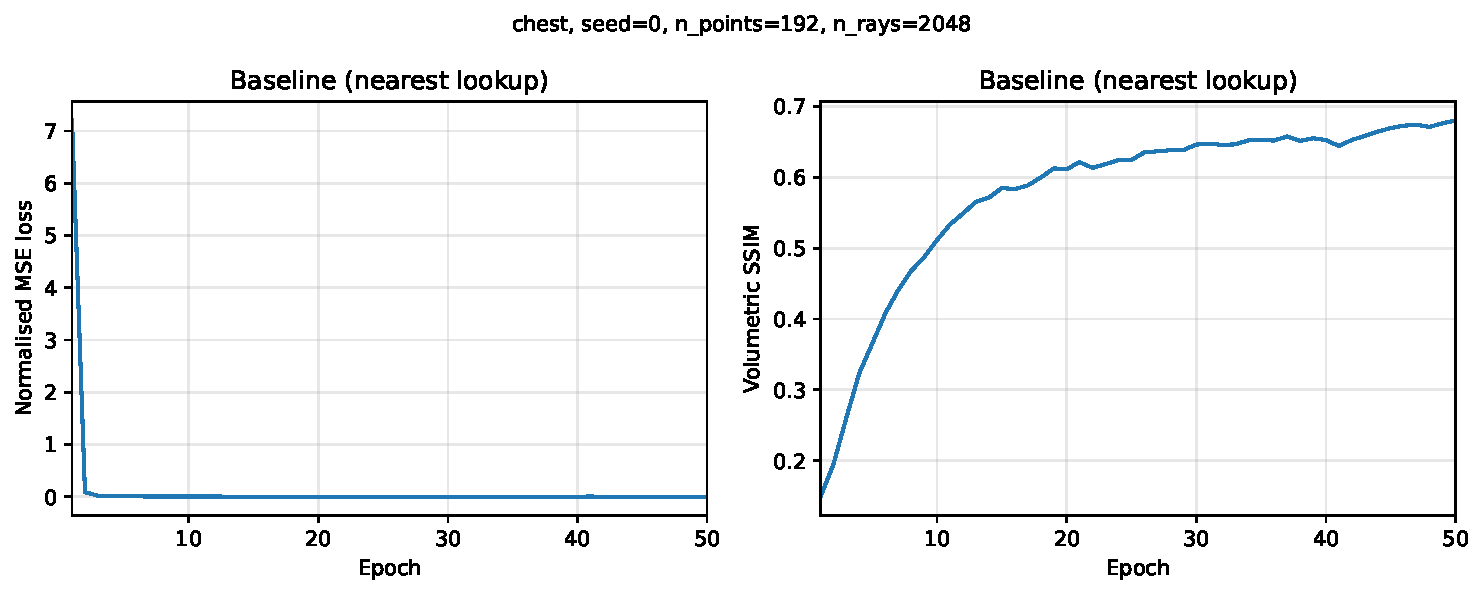
\includegraphics[width=\textwidth]{figures/fig1_baseline.pdf}
  \caption{Baseline (nearest lookup) on chest, seed~0, \(n_{\mathrm{points}}=192\), \(n_{\mathrm{rays}}=2048\).
  Left: normalised MSE. Right: volumetric SSIM on max-normalised \texttt{uint8} volumes.}
  \label{fig:baseline}
\end{figure}

Figure~\ref{fig:comparison} compares nearest and trilinear lookup.
[Placeholder: state the sign of the epoch-50 SSIM gap (positive, negative, or neutral) and the epoch at which trilinear SSIM first matches the nearest epoch-50 SSIM, or that it does not.]

\begin{figure}[ht]
  \centering
  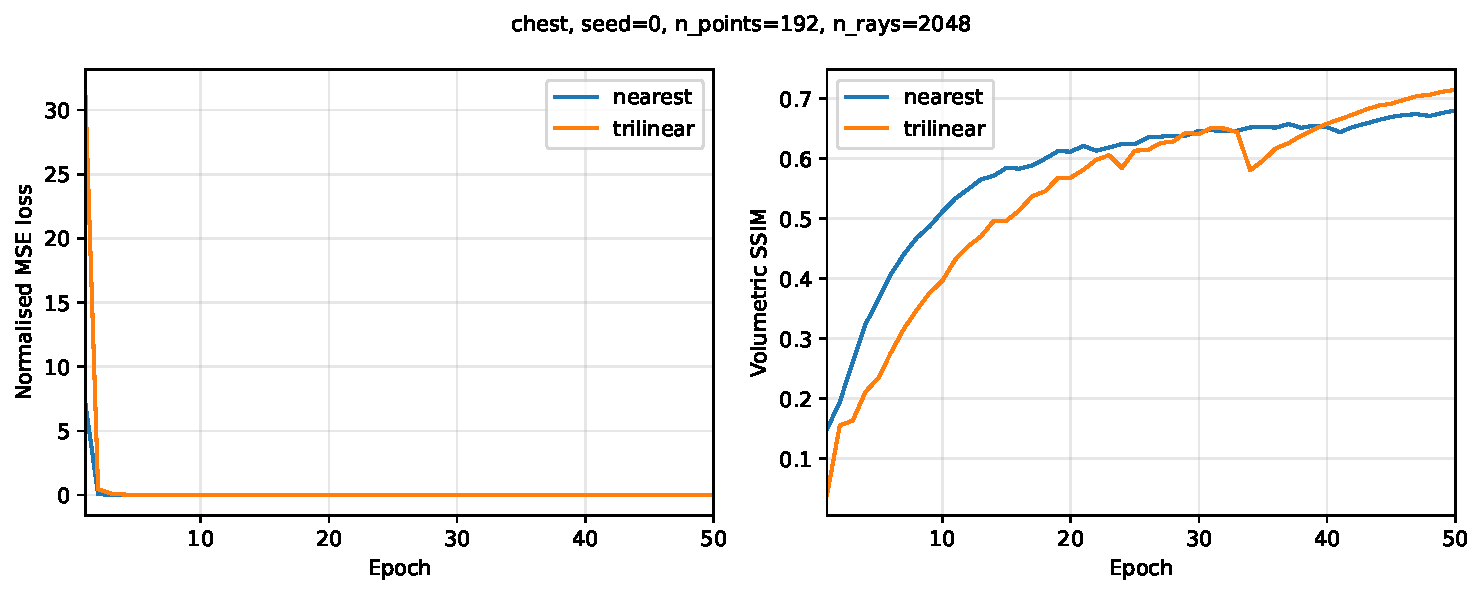
\includegraphics[width=\textwidth]{figures/fig2_comparison.pdf}
  \caption{Nearest versus trilinear lookup on the same chest protocol and seed.
  Left: normalised MSE. Right: volumetric SSIM.}
  \label{fig:comparison}
\end{figure}

\begin{table}[ht]
  \centering
  \caption{Parameter count and lookup cost. Dense multiply-adds per query point are the same for both models.}
  \label{tab:cost}
  \begin{tabular}{lrr}
    \toprule
    & Nearest & Trilinear \\
    \midrule
    Trainable parameters & XX & XX \\
    Embedding lookups per point & 8 & 64 \\
    Dense multiply-adds per point & 576 & 576 \\
    \bottomrule
  \end{tabular}
\end{table}

[Placeholder: one sentence on wall-clock time per epoch, as a secondary note only.]

\section{Conclusions}
[Placeholder: whether the hypothesis was supported, tied to piecewise-constant versus interpolated embeddings.]
Limitations: a single seed, the chest dataset only, SSIM after per-volume maximum normalisation, a 50-epoch budget, and possible GPU non-determinism.
[Placeholder: one implication for similar lookup-based reconstructions, and one future direction such as a hash encoder~\cite{zha2022naf}, a second anatomy, or more than one seed.
Gaussian embeddings~\cite{3dgrct2024} are a separate representation and were not tested.]

\bibliographystyle{plainnat}
\bibliography{refs}

\end{document}
